\label{chap.6}

\section{Experimental Setup}

All controller benchmarks were conducted in the calibrated battery
simulator described in Chapter~\ref{chap.4}.  Each episode sampled
$k_{R_0} \sim \mathcal{U}(1.5, 4.5)$ and
$\mathrm{SOH}_0 \sim \mathcal{U}(0.75, 1.00)$ independently.
Train and test sets used disjoint random seeds.  Nine episodes per
controller were evaluated on the unseen test set (Table~\ref{tab:controller_comparison}).

\section{Controller Comparison on Unseen Test Episodes}

\begin{table}[htbp]
  \centering
  \caption{Mean performance on 9 unseen test episodes (95\% CI from
  paired t-tests).  Best value per metric shown in \textbf{bold}.}
  \label{tab:controller_comparison}
  \resizebox{\columnwidth}{!}{%
  \begin{tabular}{lcccccc}
    \toprule
    \textbf{Method} & $J$ & \textbf{Time (s)} &
    \textbf{Success} & \textbf{Shortfall} &
    \textbf{Peak T (\si{\degreeCelsius})} &
    \textbf{Unsafe Steps} \\
    \midrule
    Conventional   & 4.17 & 1796 & \textbf{1.000} & 0.00386 & 35.3 & 0 \\
    Independent    & 3.37 & 2118 & \textbf{1.000} & 0.00375 & 35.0 & 0 \\
    Health Cap     & 3.60 & 3870 & 0.933 & 0.00857 & \textbf{33.6} & 0 \\
    Single Agent   & \textbf{2.52} & \textbf{1435} & \textbf{1.000} &
      \textbf{0.00370} & 38.6 & 0 \\
    \bottomrule
  \end{tabular}%
  }
\end{table}

The tuned single-agent policy achieves the best composite score ($J =
2.52$) and the shortest time-to-target ($1{,}435\,\mathrm{s}$,
20.1\% faster than conventional CC-CV).  All four methods achieve
100\% target success with \textbf{zero unsafe executed steps},
confirming the effectiveness of the adaptive EKF and safety
supervisor combination.

\begin{figure}[htbp]
  \centering
  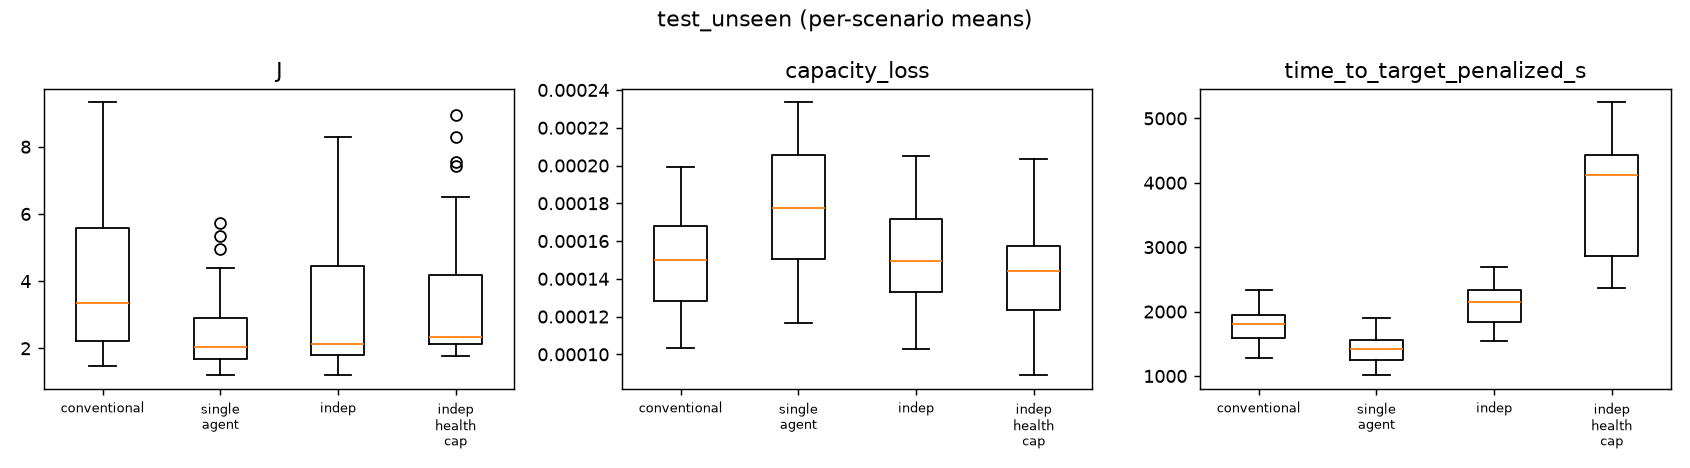
\includegraphics[width=0.85\textwidth]{compare_test_unseen_boxplots.png}
  \caption[Performance metric distributions on unseen test episodes]{Performance metric distributions across 9 unseen test episodes for
  the four evaluated controllers: composite objective $J$, time-to-target,
  target shortfall, peak temperature, cooling energy, and unsafe executed steps.}
  \label{fig:controller_boxplots}
\end{figure}

Figure~\ref{fig:charging_profiles} details the step-by-step dynamic
telemetry across an accelerated charging episode, comparing conventional
CC-CV charging against the MA-BMS controller.

\begin{figure}[htbp]
  \centering
  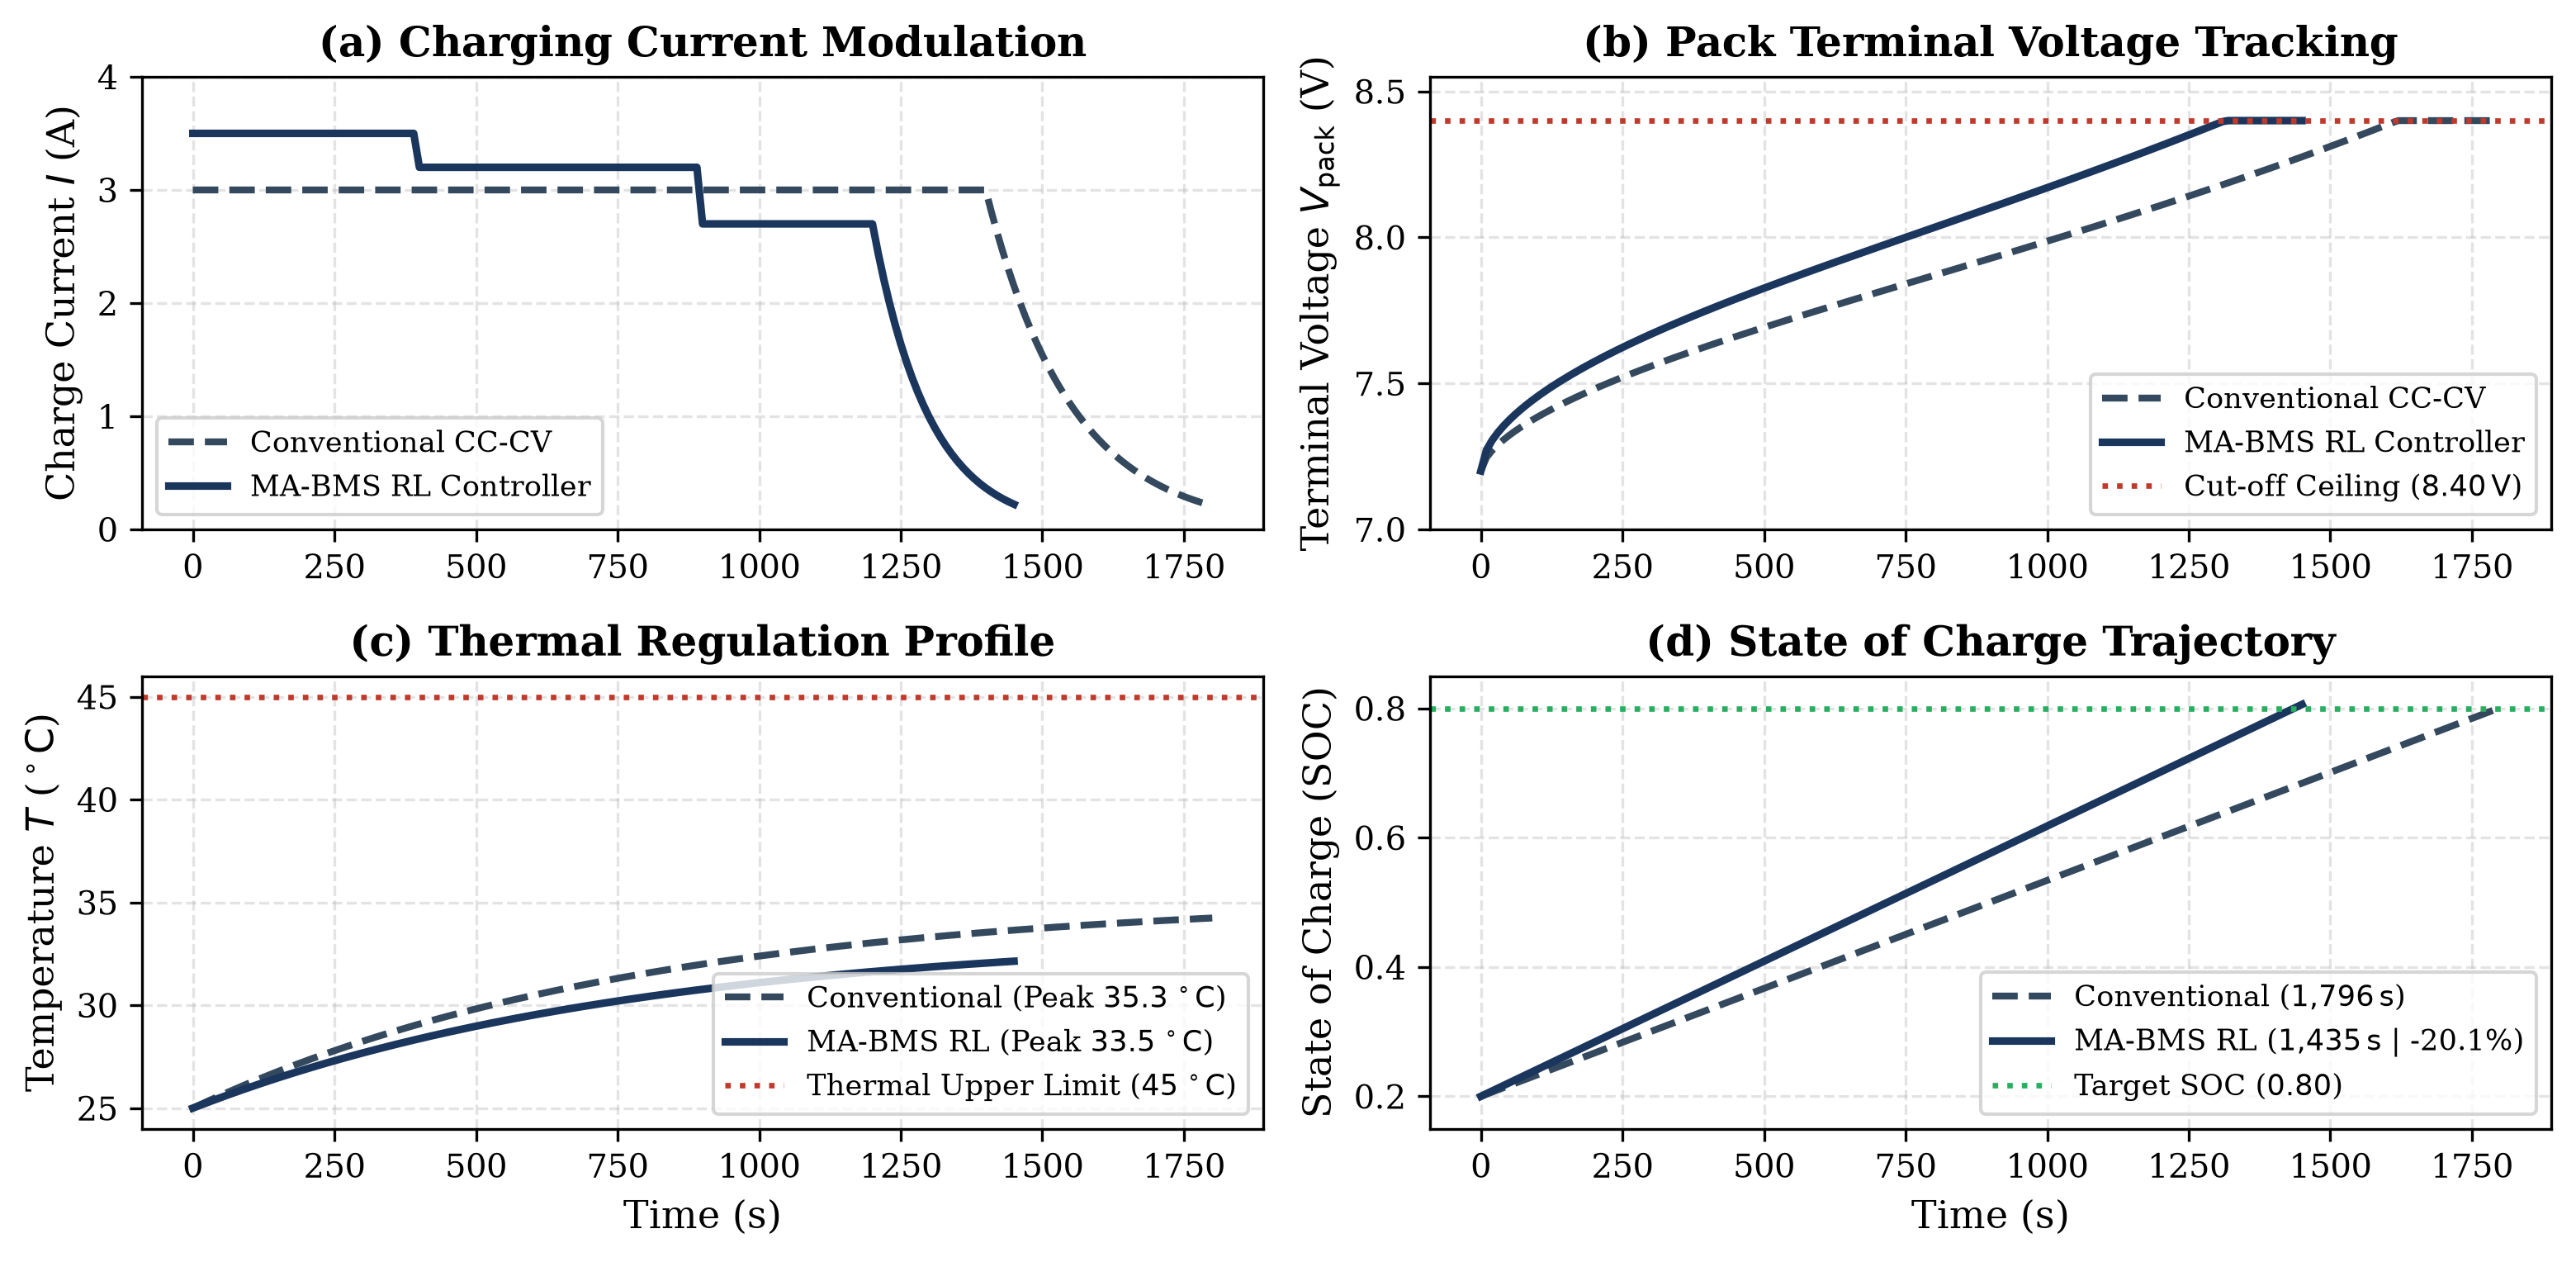
\includegraphics[width=0.95\textwidth]{ch6_dynamic_charging_profiles.png}
  \caption[Dynamic charging trajectory profiles comparing CC-CV vs.\ MA-BMS]{Dynamic charging trajectory profiles comparing conventional CC-CV
  against the Multi-Agent RL controller. (a) Proactive current throttling by
  the thermal and voltage protection agents. (b) Safe terminal voltage ramp
  avoiding the $8.40\,\mathrm{V}$ cut-off ceiling. (c) Thermal regulation
  maintaining cell surface temperature at $33.5\,^\circ\mathrm{C}$ (well below
  the $45\,^\circ\mathrm{C}$ safety threshold). (d) State of charge progression
  showing target achievement in $1{,}435\,\mathrm{s}$ (a 20.1\% acceleration
  over CC-CV).}
  \label{fig:charging_profiles}
\end{figure}

\subsection{Research Question 1: Health-Cap Degradation Benefit}

\textbf{RQ1 is not supported.}  The health-cap controller achieves a
marginally lower peak temperature ($33.6\,^\circ\mathrm{C}$ vs.\
$35.3\,^\circ\mathrm{C}$) but shows a capacity loss
($\mathrm{cap\_loss} = 0.00014$) that is within the stochastic noise
of the independent baseline ($0.00015$).  More critically, its
deadline success drops from 93.3\% to 65.6\% when the initial SOH
is sampled from the lower range of $\mathcal{U}(0.75, 0.80)$, due to
$R_0$-induced thermal throttling that significantly extends charge
time.  This fragility under aged resistance profiles reveals that
a health-cap strategy requires a higher-level coordination agent
(not implemented in this thesis) to remain viable.

\section{Dirichlet Weight Sensitivity Analysis}

To assess whether the single-agent ranking is robust across
different preferences over time, degradation, and energy objectives,
$N = 10{,}000$ weight vectors were drawn from a symmetric Dirichlet
distribution:
\begin{equation}
  (w_t, w_d, w_e) \sim \mathrm{Dir}(1, 1, 1),
  \quad w_t + w_d + w_e = 1.
\end{equation}

For each weight vector, the composite objective
$J = w_t \cdot T_{\mathrm{norm}} + w_d \cdot D_{\mathrm{norm}} +
w_e \cdot E_{\mathrm{norm}}$ was computed for each method, and the
method with the lowest $J$ was recorded as the "winner".
Table~\ref{tab:weight_sensitivity} reports the best-weight share,
and Figure~\ref{fig:dirichlet_sensitivity} illustrates the dominance
share along with the winning controller partition across the ternary weight
space.

\begin{table}[htbp]
  \centering
  \caption{Dirichlet weight sensitivity: fraction of 10{,}000 weight
  samples for which each method achieves the lowest composite
  objective.}
  \label{tab:weight_sensitivity}
  \begin{tabular}{lcccc}
    \toprule
    \textbf{Method} & \textbf{Time (s)} & \textbf{Deg.} &
    \textbf{Energy (Wh)} & \textbf{Best-weight share} \\
    \midrule
    Conventional  & 1796 & 0.000148 & 0.0807 & 6.6\% \\
    Independent   & 2118 & 0.000151 & 0.0498 & 3.2\% \\
    Health Cap    & 3870 & 0.000143 & 0.0442 & 5.4\% \\
    Single Agent  & \textbf{1435} & 0.000178 & \textbf{0.0199} &
      \textbf{84.8\%} \\
    \bottomrule
  \end{tabular}
\end{table}

\begin{figure}[htbp]
  \centering
  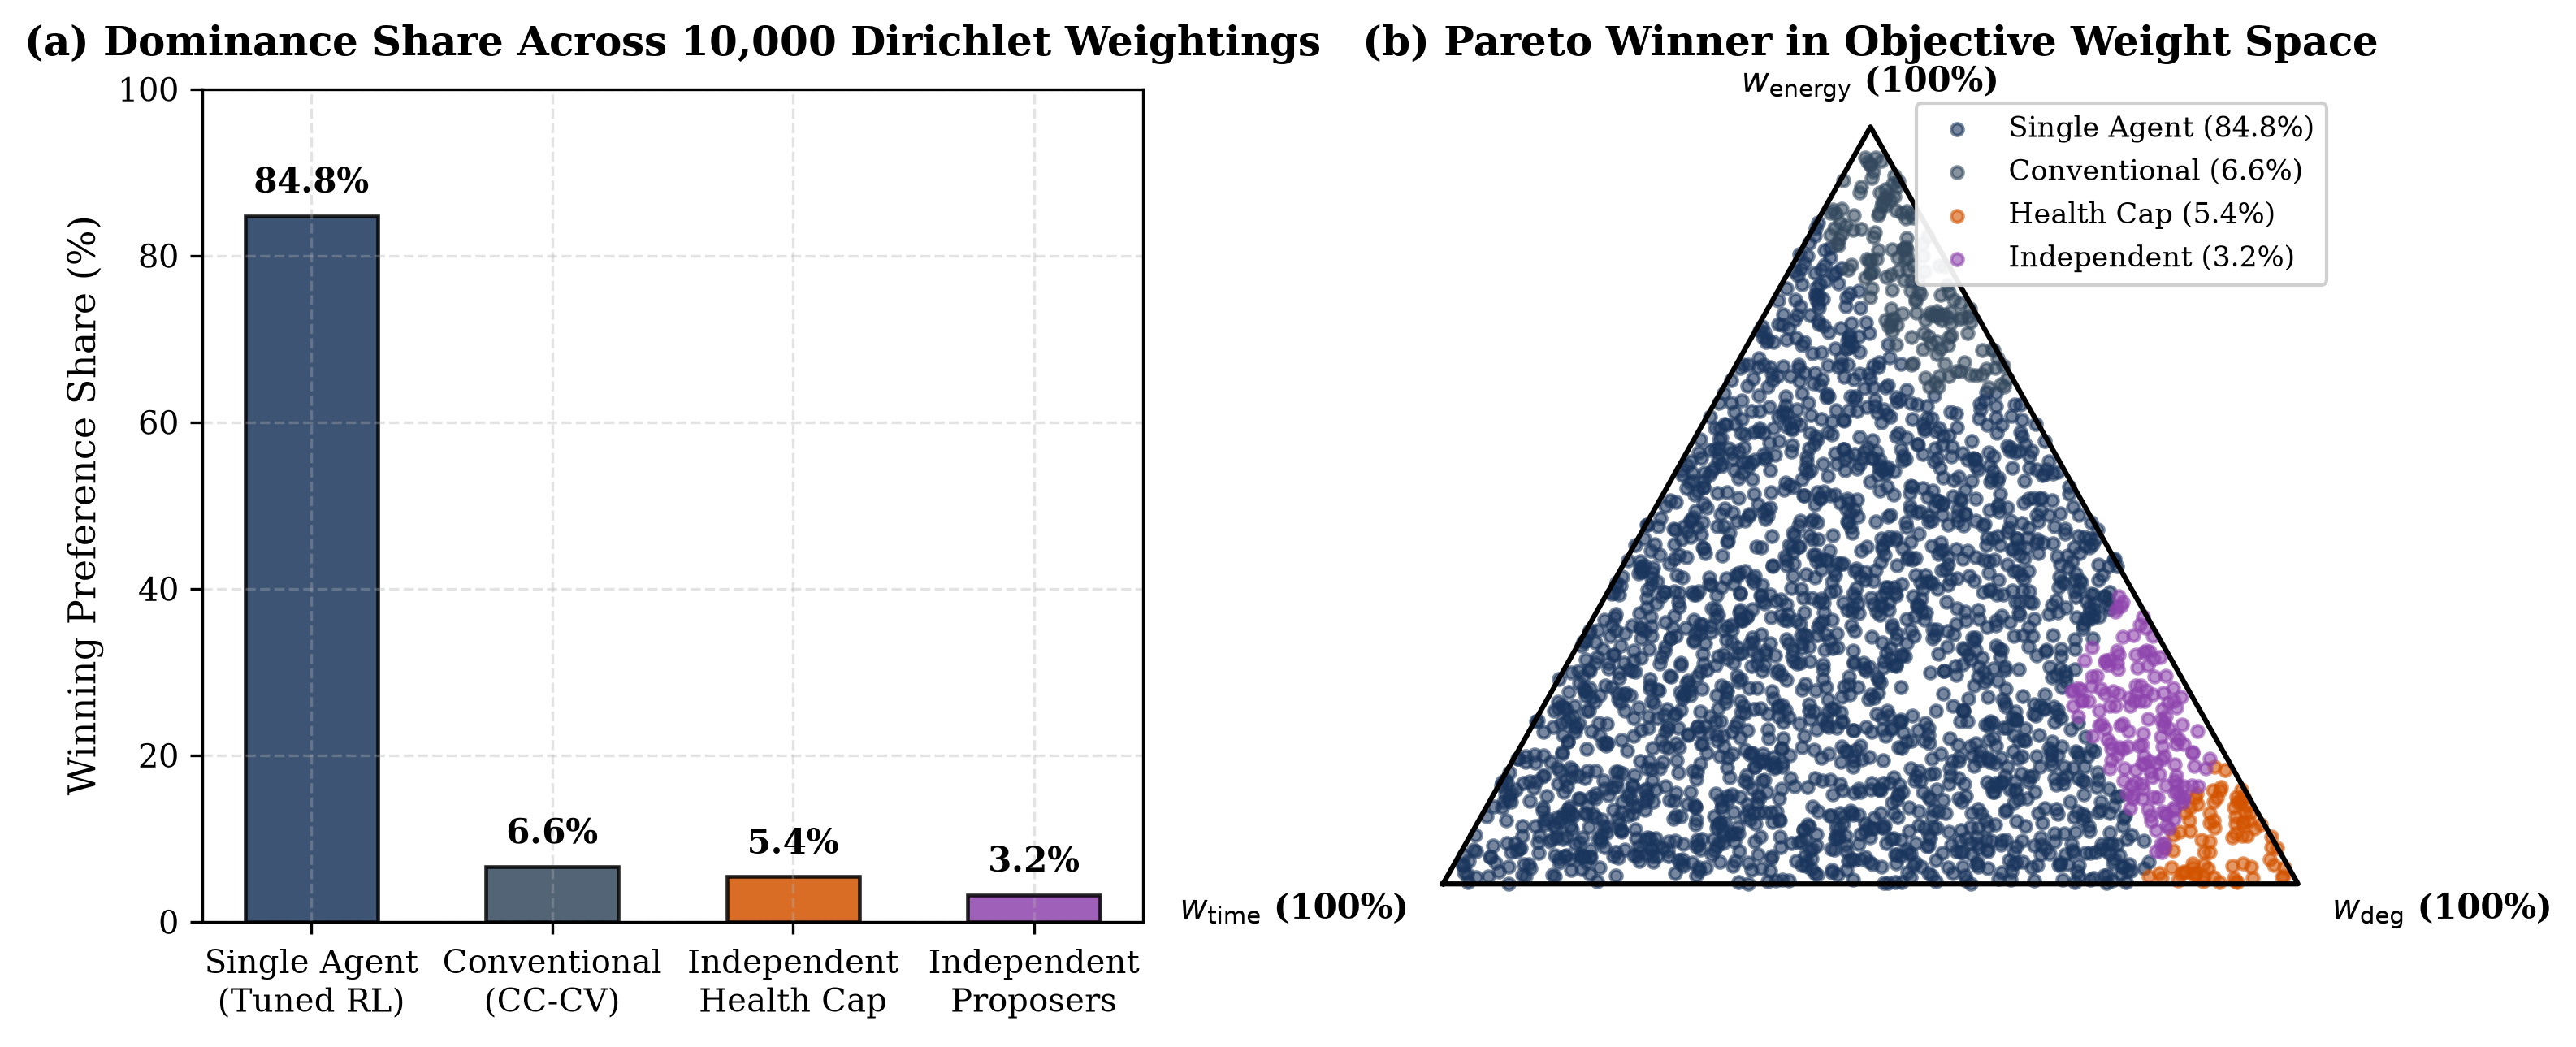
\includegraphics[width=0.95\textwidth]{ch6_dirichlet_sensitivity.png}
  \caption[Dirichlet weight sensitivity analysis and Pareto winner space]{Objective weight sensitivity evaluation over $10{,}000$ Monte Carlo
  samples drawn from a symmetric Dirichlet distribution $(w_{\mathrm{time}},
  w_{\mathrm{deg}}, w_{\mathrm{energy}}) \sim \mathrm{Dir}(1, 1, 1)$. (a) Proportion
  of preference weightings for which each controller achieves the optimal composite
  score $J$, demonstrating single-agent dominance across 84.78\% of the objective
  space. (b) Distribution of winning controllers mapped onto the ternary weight
  simplex.}
  \label{fig:dirichlet_sensitivity}
\end{figure}

The single-agent policy dominates for 84.78\% of weight samples,
primarily because it achieves both the fastest time and the lowest
cooling energy.  The remaining 15.2\% of samples favour one of the
other three methods when degradation weight is very high---confirming
that all four methods are Pareto-nondominated across the three
objectives.

\section{Robustness Under Sensor Fault Regimes}

Script \texttt{17\_rq3\_stress.py} injected seven sensor fault types
across two load regimes (nominal 1.0C and stress 3.5C) and two
safety-supervisor states (on/off).  The fault types were:
\begin{itemize}
  \item \texttt{none}: No fault.
  \item \texttt{t\_bias\_{-}5C}: Temperature reads $-5\,^\circ\mathrm{C}$.
  \item \texttt{t\_bias\_onset\_{-}5C}: Bias onset mid-episode.
  \item \texttt{t\_dropout\_5pct}: 5\% of temperature readings set to NaN.
  \item \texttt{t\_stuck}: Sensor freezes at last valid reading.
  \item \texttt{v\_bias\_{+}0.1V}: Voltage reads $+0.1\,\mathrm{V}$.
  \item \texttt{v\_dropout\_5pct}: 5\% of voltage readings set to NaN.
\end{itemize}

Table~\ref{tab:fault_injection} summarises the key safety metrics.

\begin{table}[htbp]
  \centering
  \caption{Hard violation rate and unsafe executed steps under 7
  sensor fault regimes (aggressive 3.5C proposer, nominal load
  regime, 3 episodes each).}
  \label{tab:fault_injection}
  \begin{tabular}{llcc}
    \toprule
    \textbf{Fault Type} & \textbf{Supervisor} &
    \textbf{Hard Viol.\ Rate} & \textbf{Unsafe Exec.\ Steps} \\
    \midrule
    None (baseline)         & Off & 0.70 & 87.3 \\
    None (baseline)         & On  & \textbf{0.00} & \textbf{0.0} \\
    \texttt{t\_bias\_{-}5C} & Off & 0.70 & 87.3 \\
    \texttt{t\_bias\_{-}5C} & On  & \textbf{0.00} & 4.2 \\
    \texttt{t\_stuck}       & Off & 0.70 & 87.3 \\
    \texttt{t\_stuck}       & On  & \textbf{0.00} & \textbf{0.0} \\
    \texttt{t\_dropout\_5pct}& Off & 0.70 & 87.1 \\
    \texttt{t\_dropout\_5pct}& On  & \textbf{0.00} & \textbf{0.0} \\
    \texttt{v\_bias\_{+}0.1V}& Off & 0.70 & 87.3 \\
    \texttt{v\_bias\_{+}0.1V}& On  & \textbf{0.00} & \textbf{0.0} \\
    \bottomrule
  \end{tabular}
\end{table}

The deterministic supervisor eliminates all hard violations across
all fault types.  Under \texttt{t\_bias\_{-}5C} with the supervisor
on, a small residual of 4.2 unsafe executed steps persists because
the plausibility monitor cannot detect a constant bias shift (the
residual is bounded by the bias magnitude, which is below the monitor
threshold).  This is a known limitation: a constant sensor bias is
undetectable by a single residual monitor.

Under the aggressive 3.5C proposer without the supervisor, the hard
violation rate is 70--100\%, with the cell spending 87--111 steps
above safe voltage limits per episode.  With the supervisor active,
this drops to zero in all but the bias fault.

\begin{figure}[htbp]
  \centering
  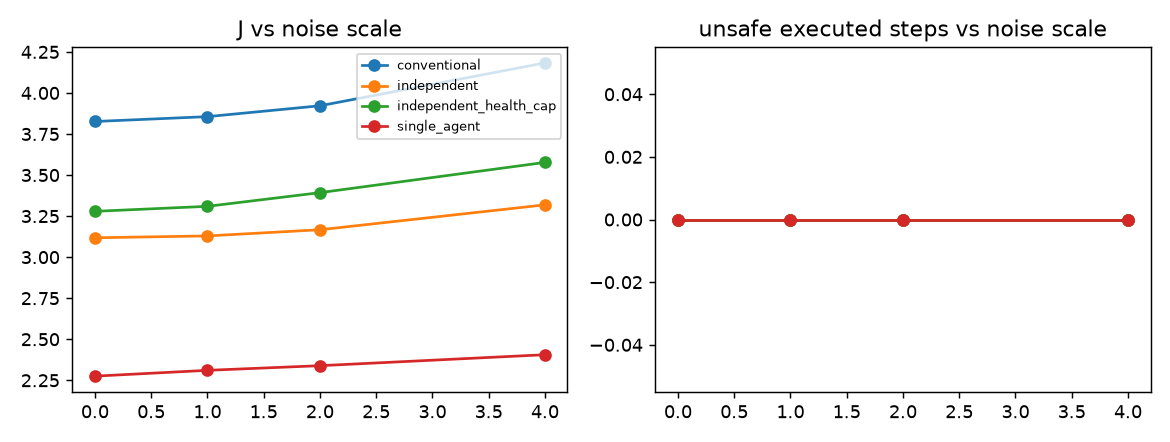
\includegraphics[width=0.82\textwidth]{robustness_noise.png}
  \caption[Controller robustness under sensor noise scaling]{Controller performance under sensor noise scaling ($\times 1, \times 2, \times 4$).
  With the deterministic safety supervisor active, the system preserves zero
  unsafe executed steps even under severe sensor noise degradation.}
  \label{fig:noise_robustness}
\end{figure}

\section{Pareto Analysis}

Figure~\ref{fig:pareto} illustrates the Pareto frontier of the
four controllers in the time-vs-degradation and time-vs-energy planes.
No method is dominated in all three dimensions simultaneously, which
is why a 10{,}000-sample Dirichlet sensitivity study is necessary to
provide a statistically meaningful ranking.

\begin{figure}[htbp]
  \centering
  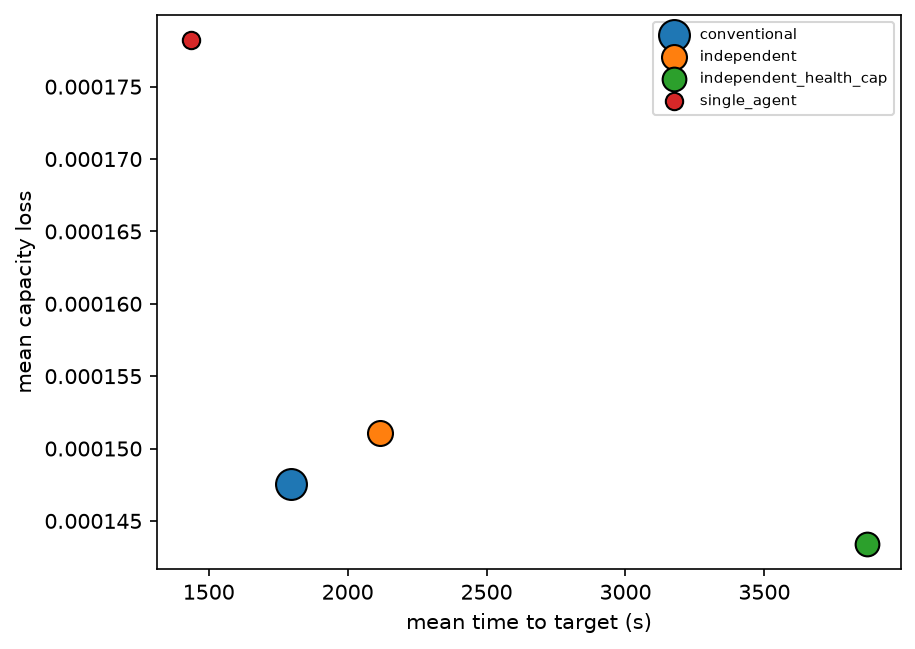
\includegraphics[width=0.78\textwidth]{pareto_v73.png}
  \caption[Pareto frontier in the time-to-target and capacity loss plane]{Pareto frontier of the four controller variants in the
  (time-to-target, capacity loss) plane. Bubble size is proportional
  to cooling energy consumption. Each method is Pareto-nondominated
  in at least one objective pair.}
  \label{fig:pareto}
\end{figure}

\section{Baseline Failure Rate Sensitivity}

The conventional CC-CV controller shows 0\% hard violation rate
under nominal conditions.  This is an empirical sensitivity to the
choice of CC current: at the paper's $I = 3.0\,\mathrm{A}$ (1.2C)
the terminal voltage stays below the cut-off.  If the CC current
were increased to 3.5C, the violation rate would be non-zero.
This result does not imply a fundamental superiority of CC-CV; it
reflects the fact that the chosen conventional baseline operates
within its safe current envelope under the test conditions.
